\chapter{A program megtervezése}
\label{chapter:program_tervezes}
\section{Az asztal felismerése}
\label{section:asztal_felismeres}

Ebben az alfejezetben a program első folyamatáról lesz szó, ami nem más mint az asztal, vagy más néven játékterület felismerése. A program ezen része bemenetként fog fogadni egy képet. Ez a kép származhat \textbf{videófelvételből} (videófelvétel egy képkockája), \textbf{valós idejű felvételből} (szintén egy képkocka), vagy szimplán egy \textbf{képfájlból}. A program bemutatásához egy felülnézetből készített snooker játszma felvételét fogom használni.
\par Az asztalfelismerő lépés kicsit elkülönül a többi lépéstől, hiszen a további lépések különféle bemenetszerzési módszerektől függetlenül, megegyezően hajtódnak végre. Ahhoz hogy a további lépések pontosak legyenek és megfeleő teljesítménnyel működjenek, az asztalt mindig azonos méretben, elforgatásban és torzításban kell megkapniuk.
\par Ebben a módszerben az elforgatást leszámítva a detektálás, átméretezés és a torzítás lesz középpontban. Az elforgatást nem veszem figyelembe, hiszen a bemenetről feltételezhető, hogy bizonyos orientációban áll rendelkezésre.

\par A valódi bemeneti kép, függetlenül annak előállítási módszerétől, a \ref{fig:bemeneti_kep} képen látható.

\begin{figure}[!ht]
    \centering
    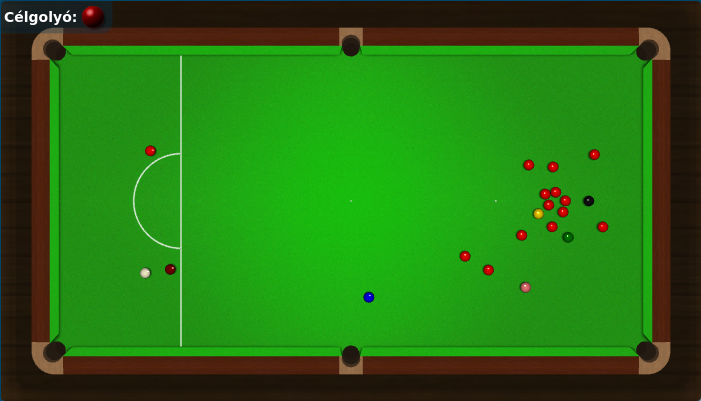
\includegraphics[width=110mm, keepaspectratio]{figures/input_screen.png}
    \caption{Egy nyers bemeneti kép a felvételről.}
    \label{fig:bemeneti_kep}
\end{figure}

\par Ezen a képen kell megtalálni a játékterület zöld részét. Ez könnyen megtehető a kép ún. HSV (Hue Saturation Value) formátumra való átalakításával. Ennek a konverziónak a kimenete a \ref{fig:bemeneti_kep_hsv} képen látható.

\begin{figure}[!ht]
    \centering
    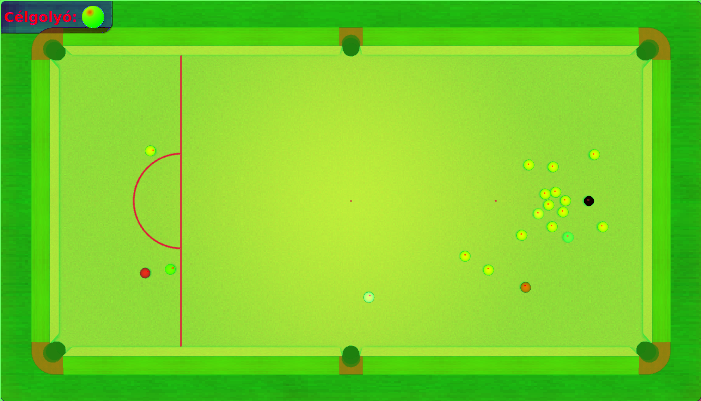
\includegraphics[width=110mm, keepaspectratio]{figures/input_screen_hsv.png}
    \caption{A \ref{fig:bemeneti_kep} kép HSV re alakított verziója RGB reprezentációban.}
    \label{fig:bemeneti_kep_hsv}
\end{figure}

\par Ez az átalakítás azért fontos, mert HSV formátumban könnyebben intervallumok közé lehet szorítani a játékterület zöld színét. A HSV konverzió belső működéséről részletesebben a megvalósítás részben lesz szó.
\newline A HSV konverzió során kapott intervallumok:
\begin{itemize}
    \setlength\itemsep{-2pt}
    \item árnyalat (Hue),
    \item telítettség (Saturation),
    \item érték (Value).
\end{itemize}

\par A HSV konverzió után az adott specifikus intervallumon kívül helyezkedő értékek maszkolásra kerülnek, hátrahagyva a kívánt játékterület képpontjait. A kép a maszkolás után visszaalakításra kerül az eredeti RGB formátumára. A folyamat után kapott kép a \ref{fig:bemeneti_kep_mask} képen látható.

\begin{figure}[!ht]
    \centering
    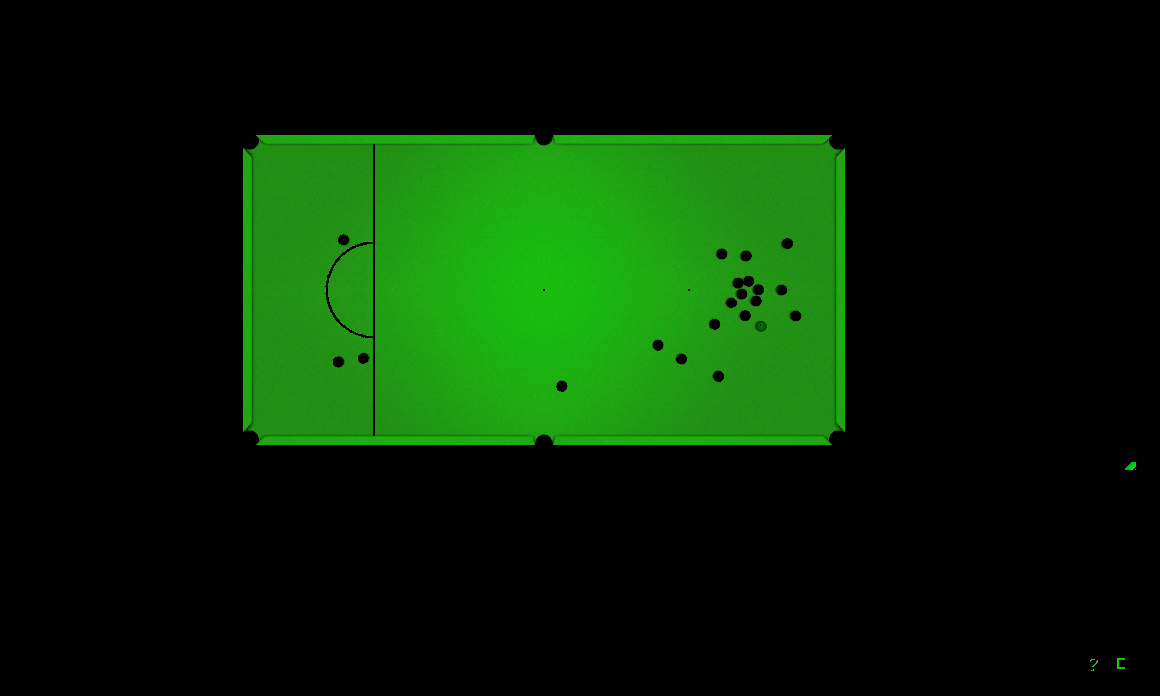
\includegraphics[width=110mm, keepaspectratio]{figures/input_screen_mask.png}
    \caption{A \ref{fig:bemeneti_kep} kép a maszkolás után.}
    \label{fig:bemeneti_kep_mask}
\end{figure}

\par Az előző folyamat után már jól látható a játékterület, azonban vannak apró foltok amik nem kerültek maszkolásra. Ezek a foltok hasonló HSV értékekkel rendelkeznek, mint a játékterület, kiszűrésük megoldható a kontúrok megkeresésével, majd feltételezve, hogy a legnagyobb folt a maszkolt képen a játékterület, annak kiválasztásával. Ezzel az eljárással már megadható a játékterület kontúrja. Szintén feltételezve, hogy ez négy sarokpontból áll, és egy téglalap pontosan határolja, a játékterület képe \ref{fig:bemeneti_asztal2} megkapható a kontúr eredeti képből való kivágásával és átméretezésével.

\begin{figure}[!ht]
    \centering
    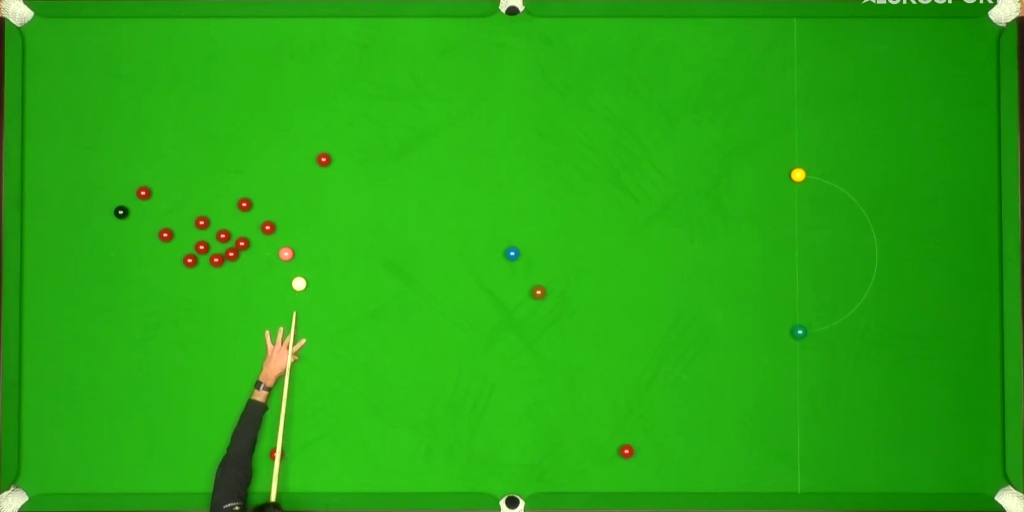
\includegraphics[width=110mm, keepaspectratio]{figures/input_table.png}
    \caption{Az eredeti képből kinyert játékterület.}
    \label{fig:bemeneti_asztal2}
\end{figure}

\par Fent említettem, hogy feltételezhető, hogy a játékterület kontúrja a kontúrkeresés után téglalap alakú, és a kontúrt alkotó pontok száma 4. Viszont valóságban ez nehezen fordul elő, ezért szükséges a pontok számának leszűkítése és a négy pontot határoló alakzatban lévő kép torzítása 2:1 oldalarányú téglalapra. Az oldalarány a szabvány snookerasztal 12 x 6 láb (365,8 cm x 182,9 cm)\cite{snooker_rules} méretéből következik. A pontok szűkítéséről és a torzításról a megvalósítás fejezetben lesz részletesetbben szó.

\section{A golyók azonosítása}
A golyók azonosítását különféle mószerekkel lehet elvégezni, ezek eltérnek sebességben és pontosságban. A folyamatok bemenete az előzőekben megismert asztal felismerés kimenete lesz, kimenetük pedig a \ref{tab:felismert_koordinatak} táblázatban látható x és y pozíciók, adott golyók színe szerint. A folyamat belső működése módszerenként eltér egymástól, ezeket a módszereket az implementáció egyes iterációjának részeként használtam, majd változtattam meg az elért teljesítmény növeléséhez.

\begin{table}[!ht]
    \caption{A golyó felismerés kimeneti adatai a \ref{fig:bemeneti_asztal2} kép alapján.}
    \label{tab:felismert_koordinatak}
	\footnotesize
	\centering
	\begin{tabular}{ l l l }
		\toprule
		golyó színe & x pozíció [0, 1023] & y pozíció [0, 511] \\
		\midrule
        fehér     & 298.5 & 283.5\\
        piros 0   & 244.5 & 204.5\\
        piros 1   & 242.5 & 243.5\\
        piros 2   & 323.5 & 159.5\\
        piros 3   & 190.5 & 260.5\\
        piros 4   & 202.5 & 222.5\\
        piros 5   & 216.5 & 259.5\\
        piros 6   & 268.5 & 227.5\\
        piros 7   & 144.5 & 192.5\\
        piros 8   & 625.5 & 451.5\\
        piros 9   & 166.5 & 234.5\\
        piros 10  & 202.5 & 247.5\\
        piros 11  & 231.5 & 254.5\\
        piros 12  & 223.5 & 234.5\\
        sárga     & 797.5 & 174.5\\
        zöld      & 797.5 & 331.5\\
        barna     & 536.5 & 291.5\\
        kék       & 512.5 & 252.5\\
        rózsaszín & 285.5 & 253.5\\
        fekete    & 120.5 & 211.5\\
		\bottomrule
	\end{tabular}
\end{table}

\subsection{Azonosítás mintaillesztéssel}
Ennek a módszernek az alapja tisztán mintaillesztéssel működik. A mintaillesztés egy arányos méretű képet illeszt rá a játékterület képére, majd amennyiben az illeszkedés mértéke meghalad egy bizonyos küszöbértéket, a mintaillesztés iterációjának a pozíciója mentésre kerül. Ebből a pozícióból meghatározható a golyó helyzete. A mintaillesztéshez használt minta a \ref{fig:minta_kep} ábrán látható.

\begin{figure}[!ht]
    \centering
    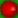
\includegraphics[width=30mm, keepaspectratio]{figures/template_red.png}
    \caption{A mintaillesztéshez használt minta.}
    \label{fig:minta_kep}
\end{figure}

\par A \ref{fig:minta_kep} minta felbontása láthatóan alacsony, azonban túl nagy felbontás esetén a folyamat meglehetősen lassabban megy végbe, továbbá a minta méretét még a felismert játékterület mérete is meghatározza.
\par A mintaillesztés problémái közé tartozik, hogy a zöld golyó mintaillesztésénél a küszöbértéket beállítani nehéz, és az eredmény pontatlan, lásd \ref{fig:rossz_zold}.

\begin{figure}[!ht]
    \centering
    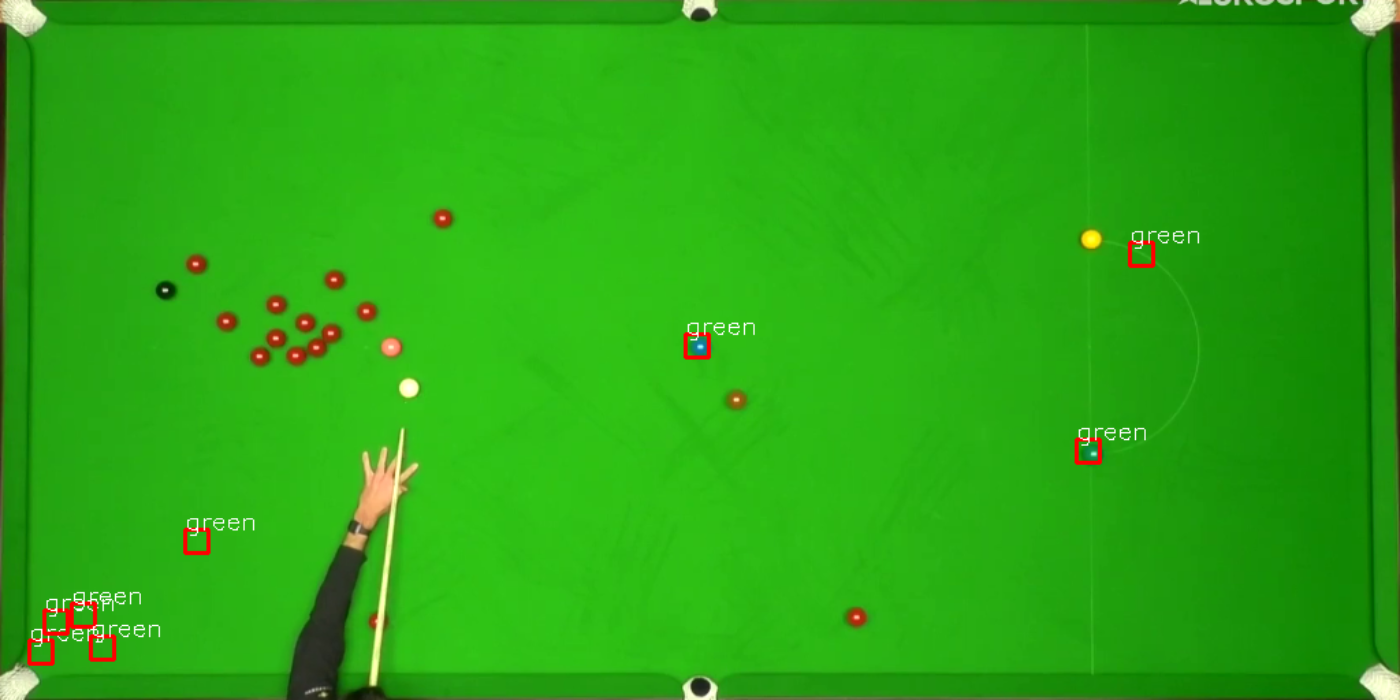
\includegraphics[width=110mm, keepaspectratio]{figures/wrong_green.png}\hspace{2mm}
	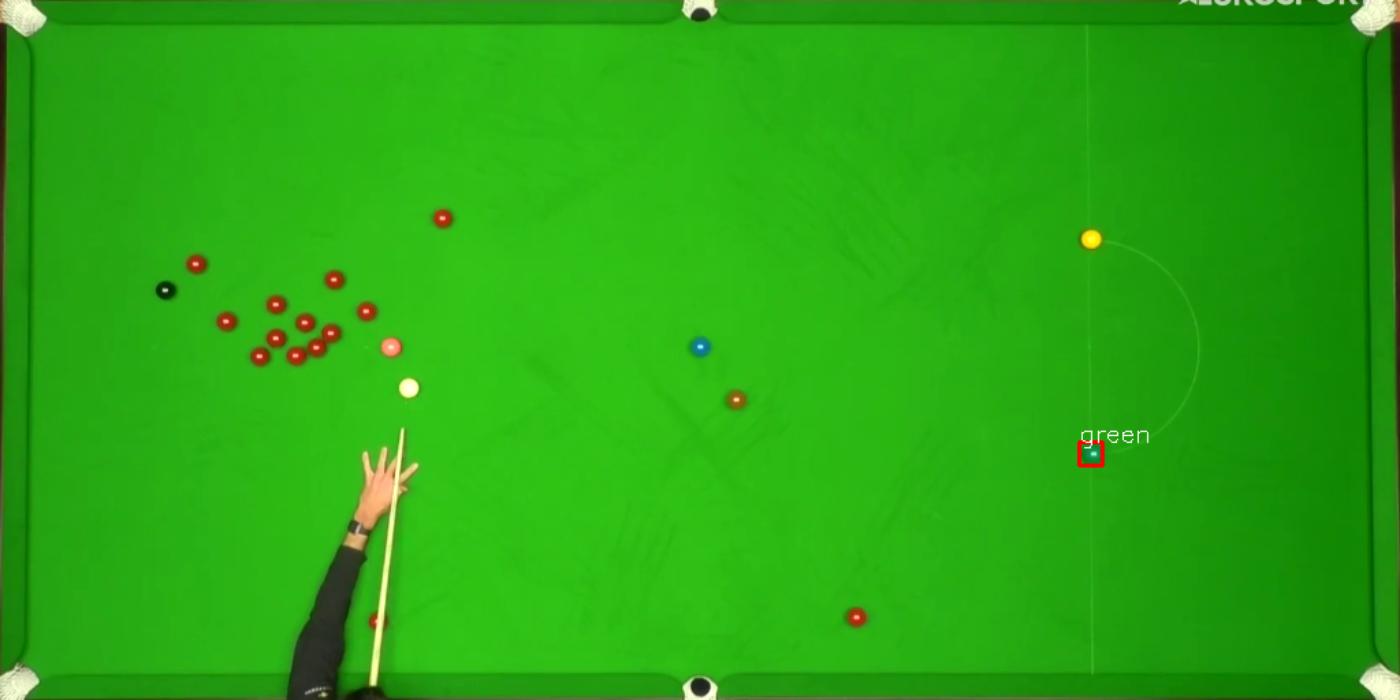
\includegraphics[width=110mm, keepaspectratio]{figures/green_ok.png}
    \caption{A zöld golyó mintaillesztésének hibája (felül) és annak orvoslása HSV konverzióval (alul).}
    \label{fig:rossz_zold}
\end{figure}

\par A \ref{fig:rossz_zold} ábrán látható hiba valamelyest orvosolható a kép és minta HSV -re való konvertálásával. Ez a konverzió jó eredményeket ad, azonban nagyon minimálisan csökkenti a teljesítményt. A mintaillesztés sajnos prolémákba ütközik a piros és barna golyók megkülönböztetésekor is. Ez a \ref{fig:rossz_barna} képen látható.

\begin{figure}[!ht]
    \centering
    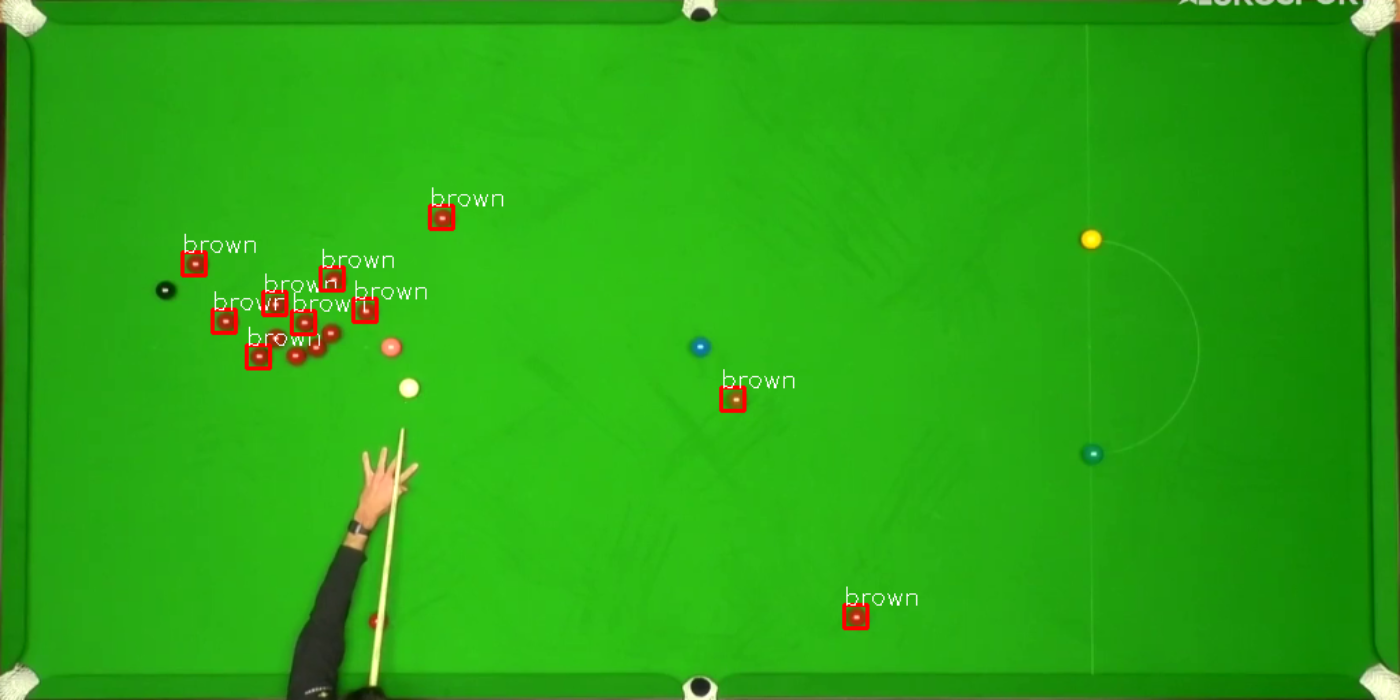
\includegraphics[width=110mm, keepaspectratio]{figures/wrong_brown.png}\hspace{2mm}
	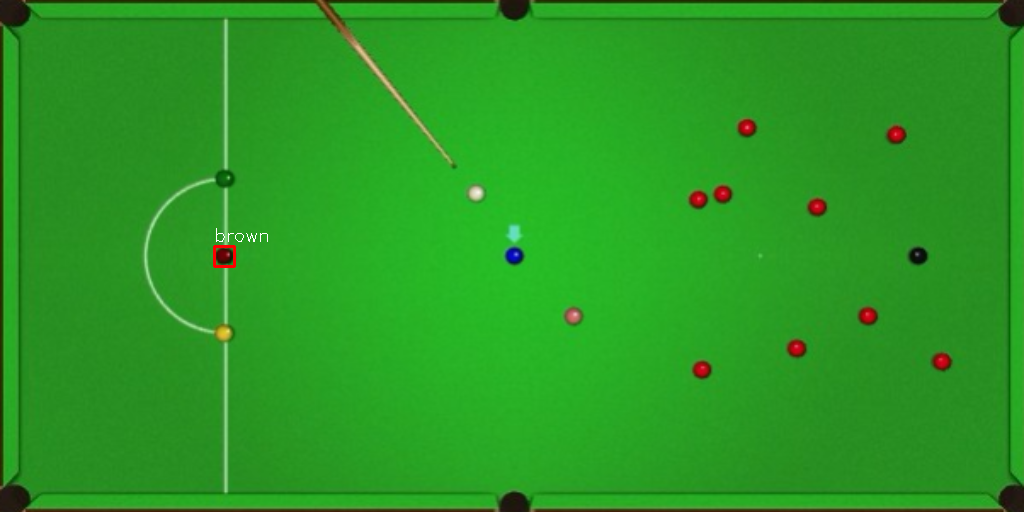
\includegraphics[width=110mm, keepaspectratio]{figures/brown_ok.png}
    \caption{A barna golyó mintaillesztésének hibája (felül) és annak orvoslása a piros golyók levonásával (alul).}
    \label{fig:rossz_barna}
\end{figure}

\par Itt a színek közelsége miatt nehéz megkülönböztetni a golyókat, ezért a piros és barna golyók nagyon minimálisan térnek el a \ref{for:cross_correlation} függvény miatt. Ez a probléma HSV konvertálás után is fennáll. Erre a megoldás, hogy az érzékelt piros golyók kivonásra kerülnek a barna golyók listájából. Ahhoz, hogy pontos legyen az eredmény, viszont szükséges, hogy a piros golyók megfelelően legyenek érzékelve, amely nem minden esetben biztosítható, ezért ez a módszer nem túl pontos bizonyos bemenetekre. Hasonló problémák merülhetnek fel a piros és rózsaszín, továbbá a fehér és rózsaszín golyók felismerésekor is.
\par Annak ellenére, hogy a módszer nem túl optimális, jól használható adatkészeletek készítésére, hiszen a felsmerést nagyrészt helyesen megoldja és a problémák ismeretében a kézzel válogatást nagymértékben megkönnyíti.

\subsection{Azonosítás körkeresés és mintaillesztéssel}
Az előző módszerhez hasonlóan a golyó színek szerinti osztályozása itt is mintaillesztéssel történik, azonban a sebesség növelése érdekében először a golyók helyzetét egy kördetektáló algoritmus határozza meg, majd a kapott értékek jutnak tovább a mintaillesztő algoritmushoz. Ez az egész képen való pásztázás és mintaillesztéshez képest a teljesítményt a minták leszűkített mennyiségének köszönhetően nagymértékben növeli.

\par A körök megtalálásához a körkereső algoritmusnak meg kell adni néhány paramétert, ezek közé tartoznak:
\begin{itemize}
    \setlength\itemsep{-2pt}
    \item a keresett körök minimális és maximális sugara,
    \item a keresett körök közti minimális távolság, duplikációk szűréséhez,
    \item az ellenőrzött alakzatok körrel való hasonlóságának küszöbértéke.
\end{itemize}
\par Az algoritmus lefutás után megadja a bemeneti játékterületen talált kör alakú kontúrokat, ezeket a \ref{fig:talalt_korok} ábra szemlélteti. A körkereső algoritmusról a megvalósítás fejezetben írok részletesebben.

\begin{figure}[!ht]
    \centering
    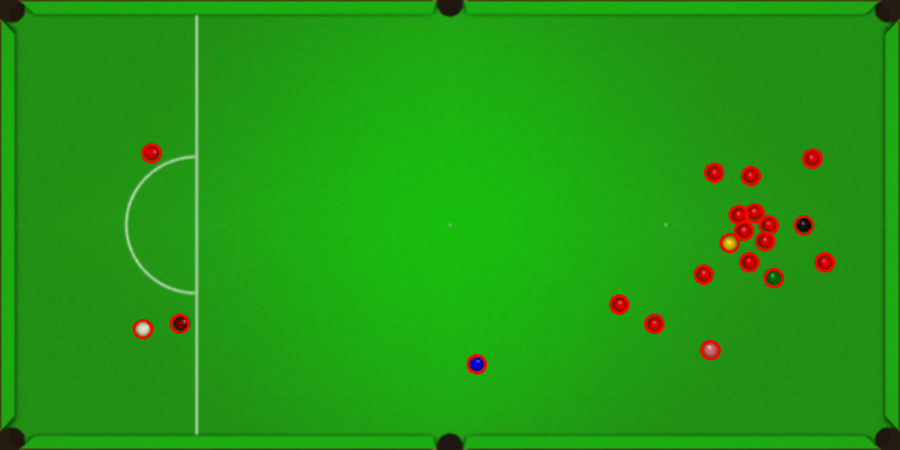
\includegraphics[width=110mm, keepaspectratio]{figures/detected_circles.png}
    \caption{A Hough transzformáció lefutása után kapott körök.}
    \label{fig:talalt_korok}
\end{figure}

\par Ez a módszer körök megtalálására jól használható, a mintaillesztéshez szükséges képek könnyedén kivághatók az eredeti képből a körök paraméterei alapján. A probléma szintén a mintaillesztéssel van, hiszen a kivágott körök az előzőleg megismert mintaillesztéssel kerülnek beazonosításra. Ez sajnos az eddig megismert hibákat vonja maga után, annak ellenére, hogy a sebesség javul. Viszont akárcsak a szimpla mintaillesztéses módszer ez a módszer is alkalmas adatkészletek elkészítésére, és a kapott adatok kézzel ellenőrzését nagymértékben megkönnyíti.

\subsection{Azonosítás körkeresés és gépi tanulás segítségével}
A mintaillesztés hibáinak kiküszöböléséhez, az osztályozás elvégezhető neurális hálózat segítségével. Ez a játékterület egy kerettel való képpontonkénti végigpásztázásával szintén megoldható, azonban körkeresésnél megismert Hough transzformációval jobb teljesítmény érhető el.

\par A következőkben a körkeresés eredményeképp kapott, a bemeneti játékterület képéből kivágott golyók osztályozásáról lesz szó neurális hálózat segítségével. A kivágott képek fogják a bemenetet képezni, majd a neurális hálózat azt osztályozza egy 0 tól 7 ig terjedő egész számként. Ezek a számok a golyók színeit reprezentálják, lásd \ref{tab:golyo_azonositok} táblázat.

\begin{table}[!ht]
    \caption{A golyók szín szerint, és azok azonosítói.}
    \label{tab:golyo_azonositok}
	\footnotesize
	\centering
	\begin{tabular}{ l c }
		\toprule
		Golyó színe & Azonosító \\
		\midrule
		fekete      & 0\\
        kék         & 1\\
        barna       & 2\\
        zöld        & 3\\
        rózsaszín   & 4\\
        piros       & 5\\
        fehér       & 6\\
        sárga       & 7\\
		\bottomrule
	\end{tabular}
\end{table}

\par A neurális hálózat betanításához szükség van betanítási adatkészletre, viszont az előzőekben megsimert módszereknél szóba került, hogy viszonylag kevés kézi szortírozással könnyedén lehet velük előállítani adatkészletet, amely tökéletes a neurális hálózat betanításához és teszteléséhez. Az adatkészlet néhány eleme a \ref{fig:adatkeszlet} ábrán látható.

\begin{figure}[!ht]
    \centering
    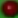
\includegraphics[width=30mm, keepaspectratio]{figures/dataset_1.png}\hspace{2mm}
    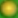
\includegraphics[width=30mm, keepaspectratio]{figures/dataset_2.png}\hspace{2mm}
	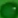
\includegraphics[width=30mm, keepaspectratio]{figures/dataset_3.png}\\\vspace{2mm}
    
\includegraphics[width=30mm, keepaspectratio]{figures/dataset_4.png}\hspace{2mm}
    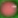
\includegraphics[width=30mm, keepaspectratio]{figures/dataset_5.png}\hspace{2mm}
	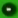
\includegraphics[width=30mm, keepaspectratio]{figures/dataset_6.png}\\\vspace{2mm}
    \caption{Az adatkészlet elemei.}
    \label{fig:adatkeszlet}
\end{figure}

\par A betöltött adatok címkével megfelelően azonosítva átadásra kerülnek a neurális hálózatnak. Ahhoz, hogy a tanítás jó eredményeket hozzon, gondoskodni kell arról, hogy a betanítási adatok közt egyenlő arányban szerepelnek az egyes golyók színek szerint, továbbá, hogy az adatkészlet elemei megfelelően össze vannak keverve. Az előkészített adatkészlet egy kis része (10\% - 30\%) elkülönítésre kerül, amely a neurális hálózat pontosságának tesztelésére fog szolgálni.
\par A betanítási folyamatok után a neurális hálózat mentésre kerül, így az későbbi kívánt használatba vétel esetén egyszerűen betölthető, a tanítás és felhasználás külön programfájlokban könnyedén elvégezhető.
\par A körfelismerés módszerrel ötvözve, a neurális hálózattal való osztályozás gyors és pontos eredményeket biztosít. A felismerés egy kimenetele a \ref{fig:felismert_asztal} képen látható.

\begin{figure}[!ht]
    \centering
    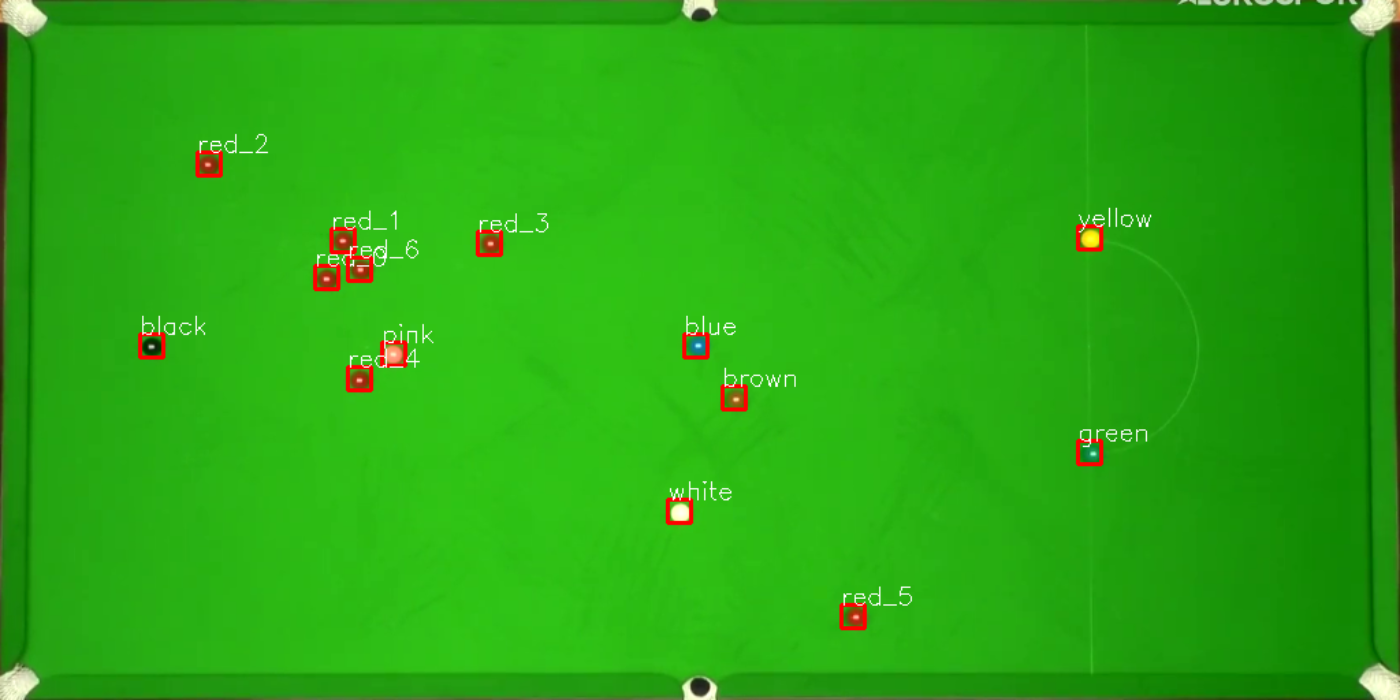
\includegraphics[width=110mm, keepaspectratio]{figures/recognised_table.png}
    \caption{A neurális hálózattal való golyófelismerés kimenete.}
    \label{fig:felismert_asztal}
\end{figure}

\par A módszer eredményességének köszönhetően későbbiekben részletesebben ismertetem a megvalósítás fejezetben.

\section{A játékmenet elemzése}
A golyók felismert pozíciója alapján a játékmenet többféle szempontból vizsgálható, ameyleknek köszönhetően érdekes statisztikai adatokhoz lehet jutni. A vizsgálati szempontok közül ebben a munkában négyfélét fogok megfigyelni, ezek az egyes golyók által \textbf{megtett távolság}, adott golyó \textbf{pillanatnyi sebessége}, a golyók \textbf{megtett útvonala} és a \textbf{zsebekben elhelyezett golyók megállapítása}.
\par Az említett szempontok alapján más komplexebb tényezőket is lehet vizsgálni (pl.: átlagos sebesség, golyók lepattanásának száma stb.), itt viszont az egyszerűség kedvéért csak az alapvetőbb szempontokat vizsgálom.
\par Ahhoz, hogy megtett utakat és sebességeket lehessen megállapítani, egy folytonos videófelvételre van szükség, a videófelvétel minősége és képkockasebessége is befolyásoló tényezők az adatok pontosságához és megállapításához.
\par A következő alfejezetekben az egyes vizsgálati szempontokat részletezem, viszont mindenek előtt még egy fontos problémának a megoldását írom le a következő fejezetben.

\subsection{A piros labdák felcímkézése}
\label{subsection:piros_labda_cimke}
A felismert golyók pozíciója és színe nagyszerű kiindulópont az egyes színű golyók útvonalának megállapításához, azonban a piros golyók sajátossága, hogy több is szerepel belőlük a játékterületen. Ez a tulajdonság ahhoz vezet, hogy az egyes golyókat meg kell különböztetni valahogy egymástól, hogy például azok útvonalát el tudjuk tárolni.
\par A probléma megoldására létezik egy elméletben viszonylag egyszerű megoldás, amely a következő lépésekből áll:

\begin{itemize}
    \item 1. Első felismerés során eltároljuk az egyes piros golyók címkéjét tetszés szerint.
    \item 2. A következő felismerési folyamat során növekvő sorrendbe helyezzük az előzőleg és jelenleg felismert piros golyók egymástól viszonyított távolságát.
    \item 3. Az előző lépésben kiszámolt listán sorban végighaladva beállítjuk a jelenlegi golyókhoz a címkét az előző golyók közül a hozzájuk legközelebb esővel.
\end{itemize}

\par A fenti módszer úgymond 'mohó' algoritmus, ezzel a számára legkedvezőbb feltételt választja minden esetben, feltételezve, hogy a golyók között a lehető legkisebb az összes elmozdulás. A módszer bizonytalannak tűnhet, azonban megfelelő minőségű videófelvétel mellett elfogadhatóan pontos eredményeket ad. A \ref{fig:felismert_asztal} ábrán látható felismert golyók ezen módszer segítségével lettek felcímkézve, és az alkalmazás megvalósításánál is a jelenlegi módszert alkalmazom.

\subsection{Megtett távolság és útvonal}
Ezt a két szempontot egy alfejezteben ismertetem, mert mindkettőjük megállapítása azonos és egyetlen alapon nyugszik, ez pedig nem más mint szimplán az adott golyók pozíciója.
\par A teljes megtett távolság könnyen megállapítható a golyók két képkocka közti elmozdulásainak a felhalmozásával. Ahhoz viszont, hogy egy számunkra hétköznapokban is használt mértékegység formájában mutatkozzanak a távolságok, egy apró trükkre lesz szükség. A golyók elmozdulásai kezdetben megállapításkor képpont formájában szerepelnek, a \ref{section:asztal_felismeres} alfejezet tábla felismerés részénél tudjuk, hogy a felismeréshez használt asztal egy fix szélességre és magasságra van transzformálva. Ennek következtében megállapítható, hogy ha a transzformációs szélesség 1024 képpont és a szabvány snooker asztal mérete a \ref{section:snooker_altalanos} rész alapján 12 láb, avagy 365,8 cm, akkor a valóságban $1\text{ cm} = \frac{1024}{365,8} \approx 2.8\text{ képpont}$ formájában mérhető a transzformált képen.
\par A megtett útvonal megállapításánál nincs szükség mértékegyésg átváltásokra, hiszen az útvonal csak a felismerés közben a transzformált asztalon kerül kirajzolásra. Az útvonal a egyes képkockákon, adott golyók pozíciójának folytonos listában való eltárolásával lehetséges. A tárolt listák közül egyet a \ref{fig:golyo_utvonal} ábrán látható módon lehet megjeleníteni a transzformált képen.

\begin{figure}[!ht]
    \centering
    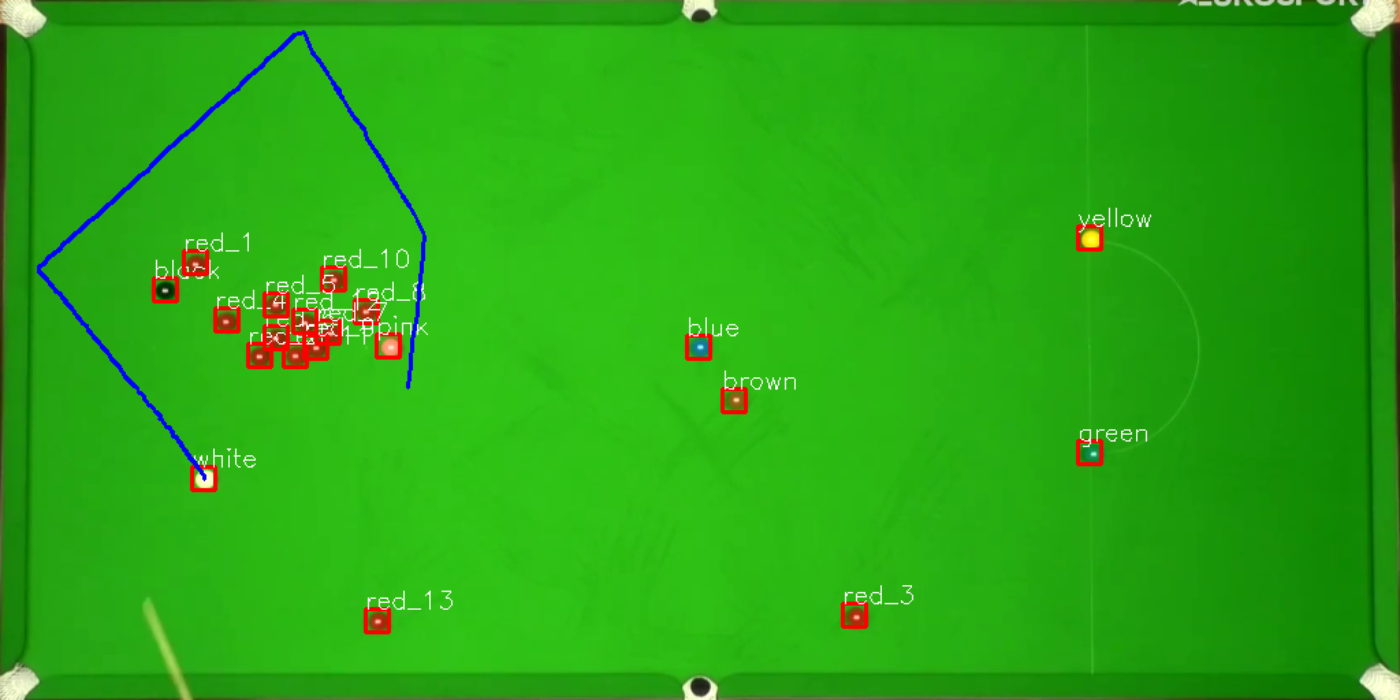
\includegraphics[width=110mm, keepaspectratio]{figures/ball_path.png}
    \caption{A fehér golyó útvonala a felismert képen kék vonallal jelölve.}
    \label{fig:golyo_utvonal}
\end{figure}

\subsection{A golyó sebessége}
Ahhoz, hogy a golyó sebességét meg lehessen állapítani, két tényezőre van szükség, ezek a megtett távolság és az ezen távolság megtételéhez szükséges idő. A megtett távolságot már az előző alfejezetben leírtak alapján megállapítható, tehát csak az eltelt időt kell kiszámolni a sebesség megállapításához. Az eltelt időt a felvétel egy paramétere, a képkockasebesség alapján fogom kiszámolni.
\par Ha a videófelvételről tudjuk, hogy a képkockasebessége 30 fps (másodpercenként 30 képkocka), vagy másnéven, két képkocka közt eltel idő $\frac{1}{30} \approx 0.03\text{ másodperc}$, és tudjuk, hogy két képkocka közt egy adott golyó elmozdulása például 3 képpont, vagy centiméterre átszámolva 1,07 cm, akkor a golyó sebessége $\frac{1,07}{0.03} \approx 35.67 \text{ cm/s}$.
\par A sebességek értékét egy listában tárolva, azokat a felismerési folyamat végén összegezve, majd leosztva a lista hosszával, kiszámolható a felismerés időtartama alatt egy adott golyóhoz tartozó átlagos sebesség.

\subsection{Zsebbe helyezés megállapítása}
A zsebbe helyezett golyó megállapítása ugyancsak a golyó pozíciójának a segítségéval állapítható meg, azonban közre játszik a feilsmert golyó beazonosításának megszakadása, megszűnése is. A golyó azonosítása akkor szűnik meg, amikor a golyó olyan takarásba vagy árnyékba kerül, hogy annak a felismerését nem lehet többé végrehajtani. Amikor egy golyó felismerése megszűnik, két képkocka közt a felismert golyók száma közt eltérés lép fel, ez visszavezethető egy adott golyóra, és annak az utolsó ismert pozíciójára.
\par Az eltűnt golyó utolsó pozíciójának ismeretében megvizsgálható annak a távolsága a zsebek pozíciójához viszonyítva. A zsebek pozíciója kiszámolható az előzőleg már említett transzformált kép tárolt fix szélesség és magasság értékeivel, hiszen a zsebek a négy sarkon és a hosszanti oldalak felénél helyezkednek el. A zsebek elhelyezkedését a \ref{tab:zsebek_kiszamolasa} táblázat szemlélteti.

\begin{table}[!ht]
    \caption{A zsebek elhelyezkedése szélesség és magasság alapján.}
    \label{tab:zsebek_kiszamolasa}
	\footnotesize
	\centering
	\begin{tabular}{ l l l l }
		\toprule
		(x, y)  & Bal           & Közép                                    & Jobb \\
		\midrule
		Alul    & (0, 0)        & ($\dfrac{\text{szélesség}}{2}$, 0)        & (szélesség, 0)\\
		Felül   & (0, magasság) & ($\dfrac{\text{szélesség}}{2}$, magasság) & (szélesség, magasság)\\
		\bottomrule
	\end{tabular}
\end{table}

\par Amennyiben a golyó utolsó ismert pozíciója elegendően közel van egy zseb pozíciójához, feltétlezhetjük, hogy a golyó az adott zsebben lett elhelyezve.